
%% bare_conf.tex
%% V1.4
%% 2012/12/27
%% by Michael Shell
%% See:
%% http://www.michaelshell.org/
%% for current contact information.
%%
%% This is a skeleton file demonstrating the use of IEEEtran.cls
%% (requires IEEEtran.cls version 1.8 or later) with an IEEE conference paper.
%%

% Keywords command
\providecommand{\keywords}[1]
{
  \small	
  \textbf{\textit{Keywords---}} #1
}

\documentclass{IEEEtran}
\usepackage[english]{babel}
\usepackage[utf8]{inputenc}
\usepackage{enumerate}
\usepackage{cite}
\usepackage{graphicx}  
\usepackage{subfig}
\usepackage{amsmath}
\usepackage{amsfonts}
\usepackage{amssymb}
\usepackage{multirow}
\pagenumbering{gobble}
\usepackage{verbatim}
\pagenumbering{arabic}
\usepackage{array}
\usepackage{hyperref}
\usepackage{svg}

% correct bad hyphenation here
\hyphenation{op-tical net-works semi-conduc-tor}


\begin{document}

%
% paper title
% can use linebreaks \\ within to get better formatting as desired
% Do not put math or special symbols in the title.
\title{Rules to Named entity recognition using evolutionary algorithm}

% author names and affiliations
% use a multiple column layout for up to three different
% affiliations
\author{\IEEEauthorblockN{Jorge Leonardo Raba\\}
  \IEEEauthorblockA{Universidad Nacional Bogotá, Colombia \\
    Email: jrabag@unal.edu.co\\
  }
}


% make the title area
\maketitle

% As a general rule, do not put math, special symbols or citationstra
% in the abstract
\begin{abstract}

  This paper describe a evolutionary algorithm to learn rules to named entity recognition (NER) using linguistic features for multiple categories. The rules extract patterns from contexts using a small corpus. The algorithm is trained with the CoNLL-2003 dataset and executed on several parallel architectures, such as distributed memory (Open MPI), shared memory (OpenMP) and hybrid (GPU) architectures. The results show that the algorithm is capable of learning rules for the recognition of named entities with high precision with a small sample size.

\end{abstract}

% explain the problem, methods and main results

\begin{keywords}
  named entity recognition, evolutionary algorithm, rule, parallel programming

\end{keywords}


\section{Introduction}

% Mini paper with Background, Problem, Method, Results and Conclusions

The named entity recognition (NER) is a sequence labeling problem where the goal is to assign a label to each word in a sentence. In order to improve the performance it often requires a large amount data \cite{ma-etal-2022-label}, which is not always available and it difficult to apply to new domains \cite{Huang2020FewShotNE}. To reduce manual effort, previous works resort to manual lexicons (Shang et al., 2018b; Peng et al.,2019) or heuristic rules provided by domain experts (Fries et al., 2017; Safranchik et al., 2020;Lison et al., 2020b) as weak supervision. However, it is challenging for experts to write complete and accurate rules or lexicons in emerging domains, which requires both a significant amount of manual effort and a deep understanding of the data.

In this work, the explored method can generate several high-precision rules for each entity, this method considers the theory proposed by Holland \cite{holland-1992-adaptation} about niche environment and speciation. The dynamics of speciation is determined by competition between niches through function sharing and migrations between islands, which causes niche formation and subdivision of the environment and population.

The islands model promotes population speciation through the formation of subpopulations isolated from each other. The subpopulations are connected by a migration operator that allows the exchange of information between them\cite{holland-1992-adaptation}. The migration operator is used to maintain population diversity and prevent premature convergence and extinction of subpopulations.

To simulate the resources in the island model, each island uses a different sentence dataset, where each island has an entity related dataset to encourage convergence of speciation around an entity. This niche approach allows individuals to take advantage of the current characteristics of the environment to quickly eliminate dominant versions of an entity, so rules that are dominant on the island of people might not perform very well on the island of organizations.

To select the best rules for each generation, first calculate the fitness that is based on the RlogF \cite{seman_lex} of the rules, then calculate the shared fitness function that helps reduce competition between individuals with a similar goal and solution different to maintain a more diverse population \cite{goldber_mul}. and finally, it uses a pseudo order, where parents compete with their children in a round-robin tournament to select the best rules. The losers can compete with the children of the neighbors to select the best rules. The pseudo order is used to avoid premature convergence of subpopulations.

In this work, the proposed method can learn the semantic and logical rules of NER using evolutionary algorithms using a small amount of labeled data. The method is trained using the CoNLL 2002 \cite{tjong-kim-sang-2002-introduction} data set. The method is implemented in several parallel architectures and the results show its scalability for shared (OpenMP), hybrid (GPU) and distributed (MPI) memory architectures. The results show that the method is capable of learning precision rules.

The paper is organized as follows. In section 2 the related work is presented. In section 3 the method is presented.
In section 4 the expetimental setup are presented. In section 5 the results are presented. In section 6 the conclusions are presented.

% no keywords


% For peer review papers, you can put extra information on the cover
% page as needed:
% \ifCLASSOPTIONpeerreview
% \begin{center} \bfseries EDICS Category: 3-BBND \end{center}
% \fi
%
% For peerreview papers, this IEEEtran command inserts a page break and
% creates the second title. It will be ignored for other modes.
\IEEEpeerreviewmaketitle


\section{Background}

\subsection{Linguistic features}

The linguistic features used are Parts of speech (also known as POS) and dependency grammar (Dep). PoS and named entities are useful clues to sentence structure and meaning. Knowing whether a word is a noun or a verb tells us about likely neighboring words (nouns are preceded by determiners and adjectives, verbs by nouns)\cite{martin-2020-speech}

A dependency grammar described relations that hold among the words, this relations provide an approximation to the semantic relationship between predicates and their arguments\cite{martin-2020-speech}

\subsection{Named entity recognition}

The named entity term named entity can be referred to with a
proper name: a person, a location, an organization, although it
is commonly extended to include things that aren't entities per se\cite{martin-2020-speech}.

The named entity recognition (NER) is a fundamental task in natural language processing (NLP) that  serves as an uptream compoment for more complex task \cite{ma-etal-2022-label}. The named entity recognition is the task of identifying and classifying the named entities in a text. The named entities are the words that refer to a person, organization, location, date, time, money, percentage, and so on.

In this task each word $x_i$ in an input word sequence, a
label $y_i$, so that the output sequence Y has the same length as the input sequence X are called sequence labeling tasks
The named entity recognition is a sequence labeling task. This sequence is the input of the named entity recognition\cite{martin-2020-speech}.


\subsection{Evolutionary algorithms}

Evolutionary algorithms are inspirated from the process of natural evolution. A given environment is filled with a population of individuals that strive for survival and reproduction. The fitness of these individuals is determined by the environment, and relates to how well they succeed in achieving their goals\cite{eiben-2015-speech}. Environment is Problem to solve, and the individuals are the solutions to the problem. The fitness function is the measure of the quality of the solution. The goal of the evolutionary algorithm is to find the best solution to the problem.

Each individual is a dual entity: its phenotypic properties (outside) are
represented at a genotypic level (inside). In other words, an individual’s genotype encodes its phenotype. Genes are the functional units of inheritance
encoding phenotypic characteristics. Here it is important
to distinguish genes and alleles. An allele is one of the possible values that
a gene can have\cite{eiben-2015-speech}

\subsection{Related work}

Historically, two major approaches have been used for entity recognition, one based on rules, the other based on statistical models. Rule-based approaches required dictionaries, regular expressions, and semantic constraints. Statistical models for named entity recognition, on the other hand, require labeled data for training purposes, as well as a statistical model that learns probabilistic representation, with collection being one of the main challenges with this approach, as the data is not always they are available and it is difficult to apply them to new domains \cite{martin-2020-speech}.

Due to the interdependence between the entities named in a piece of text, this has often been modeled as a sequence tagging task, which has proven to be an effective strategy. Early examples of this approach are hidden Markov models, maximum entropy and conditional random fields (CRFs) as is mentioned in \cite{martin-2020-speech}.

Thelen developed a weakly supervised bootstrapping algorithm  that automatically generates semantic lexicons from extraction
pattern contexts\cite{seman_lex} in 2002. Tallor \cite{tallor} is a proposed a method to learn rules using a seed rules
we propose to learn compound logical rules in 2017,

\section{PROPOSED MODEL}


\subsection{Individual encoding}

The genotype of individuals is represents using 10 double values.
. Each individual seeks to identify the sequence of vector that match with of the linguistic features in the sentences. The individual is encoded as follows:
\begin{itemize}
  \item first token: is length of the rule. Thw minimum value is 1 and maximum values is 7.
  \item  second token: is the island number that the individual belongs. The minimum value is 1 and maximum value is 8.
  \item  third token: type of entity that the rule is related to. The minimum value is 1 and maximum value is 4.
  \item  last tokens: are the tokens that the rule covers. When the rule is shorter than 7 tokens, the last tokens are filled with 0. The minimum value is 1 and maximum value is 2784.
\end{itemize}

(pending image length of entities)

The linguistic features that can have each chromosome are:
\begin{itemize}
  \item Part of Speech (PoS\footnote{https://universaldependencies.org/u/pos/}). Values between 1 and 19.
  \item Sintatic dependency (Dep\footnote{https://universaldependencies.org/u/dep/}) Values between 20 and 81.
  \item Text. Values between 82 and 2784. The value 2781 is used to unknown words.
\end{itemize}

\subsection{Island model}

Each island as you can see in figure \ref{fig:island} is evaluated with documents that have at least 1 entity recognized by the island. In this way certain individuals may have a higher fitness than others according to island where fitness is evaluated. If the individual's entity is the same as the one recognized by the island that individuals take advantage.

\begin{figure}[ht]
  \caption{Island model}
  \centering
  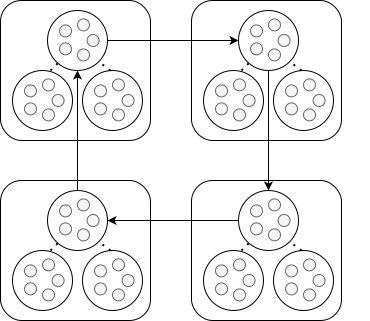
\includegraphics[width=8cm]{img/island_ae.png}
  \label{fig:island}
\end{figure}

A migration of individuals between populations is performed. The individuals that are most to the left are selected, which could be considered as those with the best fitness of the current population and are migrated to the destination population. The individual most to the left is selected that is of the same type as the individual that is to be migrated. The migrated individuals are replaced by individuals of the destination population. A migration between populations is performed every 10 generations.

\subsection{Mutation}

Three mutation operators are used:
\begin{itemize}
  \item  Gen mutation: The value of a gen is changed to a random value between 1 and 2784.
  \item Gen mutation: Two individuals are created from a parent. A gen is selected randomly and this is replaced by a gen whose value is selected randomly. One individual has a positive value and the other has a negative value.
  \item  Addition mutation: A new gen is created with a random value between 1 and 2784. The position of the new gen is randomly selected according to the size of the parent from which two individuals are created. One individual has a positive value and the other has a negative value.
  \item Deletion mutation: An individual is created from a parent. A gen is selected randomly and this is deleted from the individual. The genes that are to the right of the deleted gen are shifted one position to the left.
\end{itemize}
When a gen is created o modified, first select a linguistic feature and after select a value for the feature. For PoS the value is selected randomly between 1 and 19. For Dep the value is selected randomly between 20 and 81. For Text the value is selected randomly between 82 and 2784.


\subsection{Fitness function}

The fitness function is defined as an adaption of the
RlogF method (\ref*{RlogF_eq})\cite{seman_lex}. The fitness \ref{fitness_eq} is calculate over average of documents that contains at least one entity.

\begin{equation}
  \label{RlogF_eq}
  F(r) = \frac{F_i}{N_i} {\log_2}({F_i})
\end{equation}

\begin{equation}
  \label{fitness_eq}
  fitness = \frac{1}{N} \sum_{i=1}^{N} F(r_i)
\end{equation}

The RlogF metric is a weighted conditional probability, a pattern receives a high score if a high percentage of its extractions are category members\cite{seman_lex}. This method also considers accuracy and coverage, because $\frac{F_i}{N_i}$ represents the accuracy and ${\log_2}({F_i})$ represents the rule's ability to cover more spans \cite{tallor}

The sharing function \ref{shared_eq} use cosine distance between individuals taking from 2 token to 10 tokens. The individual fitness \ref{shared_eq_ind} is calculated in each island.

\begin{equation}
  \label{shared_eq}
  sh(d) = \left \{
  \begin{array}{l}
    1  - \frac{d}{\sigma_{share}}, d < {\sigma_{share}} \\
    0, otherwise
  \end{array}
  \right \}
\end{equation}

\begin{equation}
  \label{shared_eq_ind}
  f^t_i = \frac{f_i}{\sum_{j=1}^N sh(d_{i,j})}
\end{equation}

\subsection{Selection}

A pseudo sorting of the individuals is performed according to their fitness. The individuals with the best fitness are selected and the individuals with the worst fitness are eliminated. A tournament is held between the individuals to select the best. The tournament is held as follows: The parents and children compete with the neighbor on the right, In parent population the winner moves one place to the left, In offspring the winner moves one place to the right. In Figure \ref{fig:seudo_sort} P2 is the winner, then P1 is moved to zero position and P1 is moved to 1 position, C11 and C22 are winner then C11 is moved to position 1 and C22 kept position. To select the winner the i's parent position, then competes parent in postion i a child in position i * 2 and position i * 2 + 1. The winner stays with the position of the parent, In the figure \ref{fig:seudo_sort} C11 is winner between P2 and C21, then C11 is moved to position 0 the parent population, C11 is selected individual. The process is repeated until the population is completed.

\begin{figure}[ht]
  \caption{Pseudo sorting}
  \centering
  \includegraphics[width=8cm]{img/pseudo_sort.png}
  \label{fig:seudo_sort}
\end{figure}


\subsection{EXPERIMENTAL SETUP}

\subsubsection{Settings}

The datasets used in this paper is connll 2002\cite{tjong-kim-sang-2002-introduction}.The data represents news wire covering two languages: Spanish and Dutch. For the experiments only Spanish data is used. The data is divided into 3 sets: train, development (testa) and test (testb). The dataset is annotated by four entity types: persons (PER), organizations (ORG), locations (LOC), and miscellaneous names (MISC).

The vocabulary used is built using train dataset. A special token is added to the vocabulary to represent unknown words.The vocabulary is built using the following steps:
\begin{itemize}
  \item The words are converted to lowercase.
  \item The words with frequency less than 10 are removed.
  \item The words are sorted by frequency.
  \item The words are converted to integers starting from 1.
\end{itemize}

To train the model, the following parameters are used:
\begin{itemize}
  \item Population size: 1200
  \item Number of generations: 1000
  \item Number of islands: 8
  \item Migration interval: 10 generations
  \item 200 sentences with entities are selected randomly of train dataset.
\end{itemize}

For experiment the population is split in 8 islands. Each island has 150 individuals that recognize a person (PER), location (LOC), organization (ORG) or miscenlanius (MISC). The init population is generated with a random positive value in a first chromosome, the rest of the chromosomes will have a value of 0.

\subsection{sequential algorithm}

The secuential algorithm is implemented in C++ run in debian 11 bullseye. The algorithm is executed in a Ryzen 7 serie 4000 machine with 4 dual cores and 16GB of RAM. The algorithm is executed in 1000 generations and the time is 1039.98 seconds.

\subsection{parallel algorithm with OpenMP}

The parallel algorithm is implemented in C++ in OS is debian 11 bullseye. The algorithm is executed in a Ryzen 7 serie 4000 machine with 4 dual cores and 16GB of RAM. The algorithm is executed in 1000 generations and the time is measured in seconds. Each threads run in a island and each 10 generations the islands are migrated. The time with 8 threads is 165.76 seconds. The algorithm is executed in 1,2,3,4,5,6 and 8 threads

\subsection{parallel algorithm with cuda}

The parallel algorithm is executed in a Tesla T4 GPU with 16GB of RAM. The algorithm is executed in 1000 generations and the time is measured in seconds. This GPU has 40 multiprocessors and each multiprocessor has 64 CUDA cores. The algorithm is executed in 64,128,512,1024,2046 and 4096 threads. The cuda Capability Major/Minor version number is 7.5. Cuda version is 11.2.

Each threads run in a set of individuals. The selected function and migrate function runs in parallel. With 4069 threads the time is 11.85 seconds.

\subsection{parallel algorithm with MPI}

The parallel algorithm is implemented in C++ in OS is debian 11 bullseye. The algorithm is executed in a cluster formed with 4 machine with 2 dual cores and 4GB of RAM. The algorithm is executed in 1000 generations and the time is measured in seconds. Each core run in a island and each 10 generations the islands are migrated. The time with 8 cores is 362.80 seconds. The algorithm is executed in 1,2,3,4,5,6 and 8 cores

\subsection{RESULTS AND DISCUSSION}

\subsubsection{OpenMP}

The figure \ref{fig:openmp speed} shows the speedup of the algorithm with respect to the sequential algorithm.

\begin{figure}[ht]
  \caption{Mpi speedup}
  \centering
  \includegraphics[width=8cm]{img/speep_openmp.png}
  \label{fig:openmp speed}
\end{figure}


\subsubsection{Cuda}

The figure \ref{fig:cuda speed} shows the speedup of the algorithm with respect to the sequential algorithm.

\begin{figure}[ht]
  \caption{Cuda speedup}
  \centering
  \includegraphics[width=8cm]{img/speep_cuda.png}
  \label{fig:cuda speed}
\end{figure}

\subsubsection{MPI}

The figure \ref{fig:mpi speed} shows the speedup of the algorithm with respect to the sequential algorithm.

\begin{figure}[ht]
  \caption{Mpi speedup}
  \centering
  \includegraphics[width=8cm]{img/speep_mpi.png}
  \label{fig:mpi speed}
\end{figure}



To evaluated quality of rules the following metrics are used:
\begin{itemize}
  \item recall: Represents the recall effect of a certain class, it is to predict the correct retrieve frequency in the examples with positive samples as shown in equation \ref{recall}.
  \item precision: Represents the precision effect of a certain class, it is to predict the correct match frequency in the examples with positive samples as shown in equation \ref{precision}.
  \item f1-score: Represents the harmonic mean of recall and precision as shown in equation \ref{f1}.
\end{itemize}


\begin{equation}
  \label{recall}
  R = \frac{TP}{TP + FN}
\end{equation}

\begin{equation}
  \label{f1}
  F1-Score = \frac{2*P*R}{P + R}
\end{equation}

\begin{equation}
  \label{precision}
  P = \frac{TP}{TP + FP}
\end{equation}

\begin{table}[ht]
  \caption{Traning results}
  \centering
  \begin{tabular}{|c|c|c|c|c|}
    \hline
    \textbf{}     & \textbf{precision} & \textbf{recall} & \textbf{f1-score} \\ \hline
    \textbf{PER}  & 0.89               & 0.44            & 0.59              \\ \hline
    \textbf{LOC}  & 0.50               & 0.31            & 0.39              \\ \hline
    \textbf{ORG}  & 0.71               & 0.17            & 0.28              \\ \hline
    \textbf{MISC} & 0.90               & 0.17            & 0.28              \\ \hline
  \end{tabular}
  \label{tab:results}
\end{table}


\begin{table}[ht]
  \caption{validation results}
  \centering
  \begin{tabular}{|c|c|c|c|c|}
    \hline
    \textbf{}     & \textbf{precision} & \textbf{recall} & \textbf{f1-score} \\ \hline
    \textbf{PER}  & 0.72               & 0.32            & 0.44              \\ \hline
    \textbf{LOC}  & 0.27               & 0.19            & 0.23              \\ \hline
    \textbf{ORG}  & 0.43               & 0.10            & 0.16              \\ \hline
    \textbf{MISC} & 0.32               & 0.03            & 0.06              \\ \hline
  \end{tabular}
  \label{tab:results_validation}
\end{table}


\section{CONCLUSIONS AND FUTURE WORK}

The best acceleration is achieved with the cuda algorithm. This is because a single thread executes the mutation process for an individual, the computation of the fit function. In addition, the selection is executed in parallel, a different case than Open MPI and Open that the tournament is not executed in parallel, since the parallelism is executed at the island level.

Although the Open MP execution time is better, due to the difference in the characteristics of the machines, the difference in times is understood.

Despite Opem MPI having the worst performance in terms of execution time, the truth is that in practice it is one of the best alternatives, since it allows multiple machines to be connected, increasing parallelism that can be limited with Open Mp by the limits of the cores that a machine can reach. It also allows you to combine the parallelism that is offered by both GPU with Cuda or multi-threaded with Open MP


\bibliographystyle{unsrt}       % APS-like style for physics

\bibliography{sample}


% that's all folks
\end{document}


